% \thispagestyle{empty}
% \section*{\LARGE Acknowledgement}
% \vspace*{1cm}
% I would like to express my sincere gratitude to all those who have contributed to the completion of this project. 

% First and foremost, I extend my heartfelt thanks to my supervisor Dr.Amira Mostafa for their invaluable guidance, support, 
% and encouragement throughout this endeavor. Their expertise and insights have been instrumental in shaping the direction and quality of this work.

% I am grateful to my colleagues and peers for their camaraderie, discussions, and assistance whenever needed. 
% Their diverse perspectives have broadened my understanding and inspired new ideas.

% Last but not least, I extend my appreciation to my family and friends for their unwavering support, 
% patience, and belief in me, which have been the cornerstone of my perseverance.

% This project would not have been possible without the collective effort and support of all those mentioned above. 
% Thank you for being part of this journey and for your invaluable contributions.

% Sincerely,\\
% Ahmed Mohamed Abd-Elsalam Habib

% \newpage 
% \setcounter{page}{1}

\section{Introduction}

\begin{minipage}[t][.18\textheight]{\textwidth}
\begin{wrapfigure}{r}{0.2\textwidth}
    \begin{tikzpicture}[scale=.4]
        % Axes
        \draw[|-|] (-5,0) -- (5,0);
        \draw[|-|] (0,-5) -- (0,5);
        
        \draw[|-|] (-3,0) -- (3,0);
        \draw[|-|] (0,-3) -- (0,3);
    
        \draw[|-|] (-1,0) -- (1,0);
        \draw[|-|] (0,-1) -- (0,1);
        
        % Plot
        \draw[domain=-5:5,line width=1.5pt,smooth,variable=\x,skyblue] plot ({\x},{sin(\x r)});
        \draw[domain=.5:2.5,smooth,variable=\x,orangered] plot ({\x},{1.05});
    \end{tikzpicture}
\end{wrapfigure}
When learning calculus, you are probably accustomed to the idea of higher order derivatives 

\vspace*{1.5cm}
The first derivative $\displaystyle \dv{y}{x}$ indicates the slope of a graph.
\end{minipage}
\par
\begin{minipage}[t][.21\textheight]{\textwidth}
\begin{wrapfigure}{r}{0.2\textwidth}
    \begin{tikzpicture}[scale=.4]
        % Axes
        \draw[|-|] (-5,0) -- (5,0);
        \draw[|-|] (0,-5) -- (0,5);
        
        \draw[|-|] (-3,0) -- (3,0);
        \draw[|-|] (0,-3) -- (0,3);
    
        \draw[|-|] (-1,0) -- (1,0);
        \draw[|-|] (0,-1) -- (0,1);
        
        % Plot
        \draw[domain=-5:5,line width=1.5pt,smooth,variable=\x,skyblue] plot ({\x},{sin(\x r)});
        \draw[domain=.5:2.5,line width=1.5pt,smooth,variable=\x,orangered] plot ({\x},{sin(\x r)});
    \end{tikzpicture}
\end{wrapfigure}
.

\vspace*{1.8cm}
And the second derivative $\displaystyle \dv[2]{y}{x}$ indicates concavity
\end{minipage}



And so on calculating the $ n^{\text{th}} $ derivative of a function $\displaystyle \dv[n]{f(x)}{x}$ is taking the derivative of it $n$ times 
\[
    \underbrace{\left(\dv{}{x} \dots \dv{}{x}\right)}_{\text{n times}} f(x)
\]
And this made sense but what does it mean to take a fractional derivative
\[
    \dv[\frac{1}{2}]{f(x)}{x} = ???
\]
We're going to be exploring another branch of calculus \textbf{FRACTIONAL CALCULUS}.

The expression $\displaystyle \dv[n]{f(x)}{x}$ can have multiple 
meanings first it can be thought of as a repeated differentiation 
so if we take the $ n^{\text{th}} $ derivative of a function it means taking 
the derivative $n$ times however this only makes sense for 
positive integers if we are to extend this to other numbers 
we must think of this expression as a transformation 
something that takes in a function as an input and gives a 
function as an output 

\begin{center}
    \begin{tikzpicture}[scale=1.2]
        % Axes
        \draw[-|] (-.2,0) -- (2,0);
        \draw[-|] (0,-.2) -- (0,2);
        
        \draw[-|] (0,0) -- (1,0);
        \draw[-|] (0,0) -- (0,1);
        
        % Plot
        \draw[domain=0:1.5,line width=1.5pt,smooth,variable=\x,orangered] plot ({\x},\x*\x);
        
    
        \draw[->, line width=1.5pt,DarkGreen] (2.5,1) -- (3.5,1) node[midway,above,black] {$\displaystyle \dv{}{x}$};
    
        % Axes
        \draw[-|] (3.8,0) -- (6,0);
        \draw[-|] (4,-.2) -- (4,2);
        
        \draw[-|] (4,0) -- (5,0);
        \draw[-|] (4,0) -- (4,1);
        
        % Plot
        \draw[domain=0:2,line width=1.5pt,smooth,variable=\x,skyblue] plot ({\x+4},\x);
    
    \end{tikzpicture}
\end{center}

And not as repeated differentiation 
\\
We will look at $\displaystyle \dv[n]{f(x)}{x}$ as an operator that transforms $f$ into it's $ n^{\text{th}} $ derivative


\section{Fractional Integral}
We will start with the Fractional Integral although integrals are often harder to compute, 
but they often relate more nicely to each other and are less picky about what 
functions you throw into them. 
For example any continuous function can be integrated but NOT every continuous function can 
be differentiated. 
Like the Weierstrass function which is a continuous function that has no derivative anywhere along it due to its fractal jaggedness.
\\
Let's establish a bit of notation $If(x)$ mean the indefinite integral of the function from 0 to $x$
\[
If(x) = \int_{0}^{x} f(t) \hquad dt
\]
As we talked about earlier we can think of this as a transformation something that takes in a function and outputs a function
\begin{center}
    \begin{tikzpicture}[scale=1.2]
        % Axes
        \draw[|-|] (-1,0) -- (1,0);
        \draw[|-|] (0,-1) -- (0,1);
        
        % Plot
        \draw[domain=-1:1,line width=1.5pt,smooth,variable=\x,orangered] plot ({\x},\x*\x);
        
    
        \draw[->, line width=1.5pt,DarkGreen] (1.5,0) -- (2.5,0) node[midway,above,black] {$\int$};
    
        % Axes
        \draw[|-|] (3,0) -- (5,0);
        \draw[|-|] (4,-1) -- (4,1);
        
        \begin{scope}[scale=0.1]
        % Plot
        \draw[domain=-3:3,line width=1.5pt,smooth,variable=\x,skyblue] plot ({\x+40},\x*\x*\x/3);
        \end{scope}

    \end{tikzpicture}
\end{center}
Similar to differentiation we put an exponent like thing to denote the $ n^{\text{th}} $ integral of $f(x)$ 
\\
So for example the third integral would look something like this
\[
I^3 f(x) = \int_{0}^{x}\left[ \int_{0}^{t}\left[ \int_{0}^{s} f(u) \hquad du \right]ds \right]dt
\]
\begin{center}
    \begin{tikzpicture}[scale=1.2]
        % Axes
        \draw[|-|] (-1,0) -- (1,0);
        \draw[|-|] (0,-1) -- (0,1);
        
        % Plot
        \draw[domain=-1:1,line width=1.5pt,smooth,variable=\x,orangered] plot ({\x},\x*\x);
        
    
        \draw[->, line width=1.5pt,DarkGreen] (1.5,0) -- (2.5,0) node[midway,above,black] {$\iiint$};
    
        % Axes
        \draw[|-|] (3,0) -- (5,0);
        \draw[|-|] (4,-1) -- (4,1);
        
        
        % Plot
        % \draw[domain=-1:1,smooth,variable=\x,blue] plot ({\x+4},\x*\x*\x/3);

        \begin{scope}[scale=0.2]
            % Plot
            \draw[domain=-3:3,line width=1.5pt,smooth,variable=\x,skyblue] plot ({\x+20},\x*\x*\x*\x*\x/60);
        \end{scope}
    
    \end{tikzpicture}
\end{center}
\subsection{Cauchy's Repeated Integration Formula}
As we increase the number the expression gets more and more complicated 
But Cauchy found a way to look at 
repeated integrals like this and put it in the form of a single integral of convolution type
which is Cauchy's Formula for Repeated Integration.

First we take the integral of a function $f(t)$
\begin{figure*}[b]
    \begin{minipage}[h]{\textwidth}
        \begin{enrichment}{Augustin Louis Cauchy}{Chars/Cauchy.jpg}{2.4}{.8}{.17}
            Baron Augustin-Louis Cauchy (1789-1857) was a French mathematician and physicist 
            he's well known the most for his significant contributions in analysis, calculus, and number theory 
            although he didn't make direct contributions to fractional calculus in the way we understand 
            it today, his integral formula provided a crucial tool for mathematicians who later 
            explored this area. 
            Essentially, Cauchy's formula helped establish the foundation for defining fractional 
            differentiation and integration.
        \end{enrichment} 
    \end{minipage}
\end{figure*}
\[
    If(t) = \int_{0}^{t} f(s) \hquad ds
\]
Repeating this process gives 
\[
    I^2 f(t) = \int_{0}^{t} If(s) \hquad ds  = \int_{0}^{t}\int_{0}^{s} f(\theta) \hquad d\theta \hquad ds 
\]
\begin{minipage}[t][.18\textheight]{\textwidth}
    \begin{wrapfigure}{r}{0.2\textwidth}
        \begin{tikzpicture}
            \draw[->] (0,0,0) -- (3,0,0) node[right]{$\theta$};
            \draw[->] (0,0,0) -- (0,3,0) node[above]{$s$};
            \draw[->, blue] (0,0,0) -- (2.5,2.5,0) node[above right]{$s = \theta$};
            \draw[->, orange] (0,2.2,0) -- (2.7,2.2,0) node[right]{$s = t$};
        
            \draw[-,red] (0,1,0)--(1,1,0);
            \draw[-,red] (0,1.2,0)--(1.2,1.2,0);
        
            \fill [oblique lines] (0,1,0) -- (1,1,0) -- (1.2,1.2,0) -- (0,1.2,0);
            \fill [oblique lines] (1,1,0) -- (1,2.2,0) -- (1.2,2.2,0) -- (1.2,1.2,0);
        
            \draw[-,red] (1,1,0)--(1,2.2,0);
            \draw[-,red] (1.2,1.2,0)--(1.2,2.2,0);
        
            \draw (-.2,1.1,0) node{$ds$};
            \draw (1.1,2.4,0) node{$d\theta$};
        \end{tikzpicture}
    \end{wrapfigure}
We can interchanging the order of integration using Fubini's theorem
\[
    I^2 f(t) = \int_{0}^{t}\int_{\theta}^{t} ds \hquad f(\theta) \hquad d\theta = \int_{0}^{t}(t-\theta)f(\theta) \hquad d\theta
\]
Similarly we can get $I^3f(t)$
\begin{align*}
    I^3 f(t) &= \int_{0}^{t} \int_{0}^{s} (s-\theta)f(\theta) \hquad d\theta \hquad ds
             \\
             &= \int_{0}^{t} \frac{(t-\theta)^2}{2}f(\theta) \hquad d\theta = \int_{0}^{t} \frac{(t-\theta)^2}{2!}f(\theta) \hquad d\theta
\end{align*}
\end{minipage}

\vspace*{.3cm}
And so on we can get 
\begin{equation}
    I^n f(t) = \int_{0}^{t} \frac{(t-\theta)^{n-1}}{(n-1)!}f(\theta) \hquad d\theta \quad , \quad n=1,2,3,\dots
\end{equation}
\subsection{Riemann-Liouville Integral}
Now the real question is how do we define this formula for any positive number ?
\\
The answer lies within the gamma function $\Gamma(n)$.
\begin{figure*}[b]
    \begin{minipage}[h]{\textwidth}
        \begin{enrichment}{Bernhard Riemann}{Chars/Riemann.jpg}{2.4}{.8}{.17}
            Though he is best known for his contributions to geometry and analysis, 
            he also made huge steps in the development of fractional calculus. 
            While not published until after his death, Riemann's work explored a definition for 
            fractional integration laid the groundwork for what is now known as the Riemann-Liouville 
            fractional integral, a cornerstone of the field.
        \end{enrichment} 
    \end{minipage}
\end{figure*}
\begin{figure*}[b]
    \begin{minipage}[h]{\textwidth}
        \begin{enrichment}{Joseph Liouville}{Chars/Joseph Liouville.jpg}{2.4}{.8}{.17}
            Joseph Liouville deserves credit for sparking the entire field of fractional calculus. 
            Even earlier than Riemann, Liouville, in 1832, first proposed the idea of generalizing 
            derivatives and integrals to non-integer orders. 
            While he didn't establish a complete framework, Liouville's pioneering thought and experiment 
            opened the door for mathematicians like Riemann to develop the specific definitions and tools used in fractional calculus today.
        \end{enrichment} 
    \end{minipage}
\end{figure*}


\begin{enrichment*}{Gamma Function}
    The Gamma Function is defined as follows
    \[
    \Gamma(n) = \int_{0}^{\infty} e^{-t} t^{n-1} \hquad dt \quad , \quad \forall n>0
    \]  
    And has the following properties
    \begin{itemize}
        \item $\Gamma(n+1) = n \Gamma(n)$
        \item $\Gamma(n+1) = n!$
        \item $\Gamma(1) = 1 \quad;\quad \Gamma(\frac{1}{2}) = \sqrt{\pi} $
    \end{itemize}
    The goal of the gamma function was to define a smooth 
    curve that would go through factorial points 

    It gives us a way to extend the domain of factorials 
    from positive integers to the positive real numbers 
    and even the complex numbers for $Re(n) \notin \mathbb{Z}^- \cup \{0\} $ 
\end{enrichment*}
Since the main thing restricting the domain of a formula 
for repeated integration (2.1) is the factorial we can replace 
this with the gamma function now we can plug in any positive number 
for $n$ and get a value for this integral
\begin{equation}
    I^n f(t) = \frac{1}{\Gamma(n)}\int_{0}^{t} (t-s)^{n-1}f(s) \hquad ds \quad , \quad \forall n \in \mathbb{C} , Re(n)>0
\end{equation}
This is a valid operator this particular operator is called 
the Riemann Liouville integral or RL integral for short although 
there are many other ways of going about fractional integration 
the RL integral is probably the easiest to understand 



\begin{definition}[Riemann-Liouville Fractional Integral]
    The fractional integral of the function $f \in L_1[0, b]$ is the integral of (arbitrary) order
    $\alpha > 0$  is defined by
    \begin{equation}
        I^\alpha f(t) = \frac{1}{\Gamma(\alpha)}\int_{0}^{t} (t-s)^{\alpha-1}f(s) \hquad ds
    \end{equation}
    And we define $ I^0 f(t) = f(t)$
\end{definition}
\begin{lemma}
    The definition (2.3) of fractional integral operator is satisfied in any
    point for the continuous functions and in almost every point for the absolutely
    integrable functions. 
    i.e
    \\
    \hspace*{.3cm} 1. If $f(t)$ continuous $\Longrightarrow I^\alpha f(t)$ exist $\forall t \in [0, b]$
    \\
    \hspace*{.3cm} 2. If $f(t)$ absolutely integrable ($\in L_1[0, b]$) $\Longrightarrow I^\alpha f(t)$ exist a.e (almost everywhere)
\end{lemma}

In case $\alpha > 1$ the integral $I^\alpha f(t)$ exist $\forall t \in [0, b]$ since the integrand is a product 
of an integrable function $f(t)$ and continuous function $(t-s)^{\alpha-1}$

In case $ 0 < \alpha < 1$ we can rewrite $I^\alpha f(t)$ as following
\[
    I^\alpha f(t) = \frac{1}{\Gamma(\alpha)}\int_{-\infty}^{\infty} \psi(t-s)f(s) \hquad ds  = \frac{1}{\Gamma(\alpha)} \psi(t) * f(t)
\]
Where 
    \(
    \psi(u) = 
    \begin{cases}
        \displaystyle u^{\alpha-1}  &u \in [0,b]
        \\
        \displaystyle 0  &\text{ else } 
    \end{cases}
    \)
    \\\\
Now from lemma 2.1 and Young's convolution inequality we get the following results
\vspace*{-.2cm}
\begin{result}
    If $f,\psi \in L_1 \Longrightarrow \psi * f \in L_1$ exist a.e
\end{result}
\vspace*{-.2cm}
\begin{result}
    If $f \in C \quad,\quad \psi \in L_1 \Longrightarrow \psi * f \in L_\infty$ exist $\forall$points
\end{result}

\begin{enrichment*}{Young's Convolution Inequality}
    Suppose that $f,g$ are two functions such that $f \in L_p[\mathbb{R}^d]$ and 
    $g \in L_q[\mathbb{R}^d]$ Then 
    \[
    ||f*g||_{r} \leq ||f||_{p} \hquad ||g||_{q}
    \]
    i.e $f*g \in L_r[\mathbb{R}^d]$
    where
    \begin{equation}
        \frac{1}{p} + \frac{1}{q} = \frac{1}{r} + 1 \quad ; \quad p,q,r \in [1,\infty]
    \end{equation}
\end{enrichment*}
In particular 
\\
1. If $p \hquad,\hquad q = 1$ we get that $r=1$ (Result 1)
\\
2. If $p = \infty \hquad,\hquad q = 1$ we get that $r=\infty$ (Result 2)

Now in case $ 0 < \alpha < 1$ we get that $\displaystyle \int_{0}^{b} |\psi(s)| \hquad ds < \infty \Longrightarrow \psi \in L_1[0, b]$
\begin{example}
    Evaluate $I^{\alpha}(f(t))$ where $f(t) = c$ ((Constant function))
    
    \textit{ \textbf{Sol.} }
    \begin{align*}
        I^{\alpha} (c) &= \frac{1}{\Gamma(\alpha)}\int_{0}^{t} (t-s)^{\alpha-1} \hquad c \hquad ds     
         \\
         &= \frac{c}{\Gamma(\alpha)} \left[ \frac{(t-s)^{\alpha}}{\alpha}\right]_{0}^{t}
         \\
         &= \frac{c \hquad t^\alpha }{\Gamma(\alpha+1)}
    \end{align*}
\end{example}
\begin{example}
    Evaluate $I^{\alpha}(f(t))$ where $f(t) = t^{n} \quad,\quad n>-1$ (to make sure $\Gamma$ is defined)
    
    \textit{ \textbf{Sol.} }
    \begin{align*}
        I^{\alpha}(t^{n}) &= \frac{1}{\Gamma{(\alpha)}} \int_0^t (t-s)^{\alpha-1} \hquad s^n \hquad ds
        \\
    \intertext{
            Substitute
    \(
    \begin{cases}
        \displaystyle s = t\theta
        \\
        \displaystyle ds = t \hquad d\theta
        \\
        \displaystyle 0 \to 1
    \end{cases}
    \)
        }
                          & = \frac{1}{\Gamma{(\alpha)}} \int_0^1 (t-t\theta)^{\alpha-1} (t\theta)^n \hquad t \hquad d\theta 
                          \\
                          & = \frac{1}{\Gamma{(\alpha)}} t^{n+\alpha} \int_0^1 (1-\theta)^{\alpha-1} (\theta)^n \hquad d\theta             
                          \\
                          & = \frac{1}{\Gamma{(\alpha)}} t^{n+\alpha} \beta{(\alpha,n+1)}
                          \\
                          & = \frac{1}{\Gamma{(\alpha)}} t^{n+\alpha}\frac{\Gamma{(\alpha)}\Gamma{(n+1)} }{\Gamma{(n+\alpha+1)} } 
                          \\
                          & =  t^{n+\alpha}\frac{\Gamma{(n+1)} } {\Gamma{(n+\alpha+1)} }
    \end{align*}
\end{example}
\begin{enrichment*}{Beta Function}
    The Beta Function is defined as follows
    \[
    \beta(\alpha,\gamma) = \int_{0}^{1} (1-t)^{\gamma-1}t^{\alpha-1} \hquad dt
    \]  
    And has the following property
    \begin{itemize}
        \item $\displaystyle \beta(\alpha,\gamma) = \frac{\Gamma{(\gamma)}\Gamma{(\alpha)} }{\Gamma{(\gamma + \alpha)} } $
    \end{itemize}
\end{enrichment*}

\newpage
We can do a test to show that this formula is sensible applying a 
half-integral twice should have the same effect as a regular single integral.
\begin{example}
    Evaluate $I^{\frac{1}{2}}I^{\frac{1}{2}}(f(t))$ where $f(t) = t^{n} \quad,\quad n>-1 $ 
    
    \textit{ \textbf{Sol.} }
    \begin{align*}
        \because I^{\alpha}(t^{n}) &=  t^{n+\alpha}\frac{\Gamma{(n+1)} } {\Gamma{(n+\alpha+1)} }
        \\
        I^{\frac{1}{2}}I^{\frac{1}{2}}(t^{n}) &=  I^{\frac{1}{2}}\left[ t^{n+\frac{1}{2}}\frac{\Gamma{(n+1)} } {\Gamma{(n+\frac{3}{2})} }\right]
        \\
        &=  \frac{\Gamma{(n+1)} } {\Gamma{(n+\frac{3}{2})} } I^{\frac{1}{2}}\left[ t^{n+\frac{1}{2}}\right]
        \\
        &= \frac{\Gamma{(n+1)} } {\Gamma{(n+\frac{3}{2})} } t^{n+\frac{1}{2}+\frac{1}{2}}\frac{\Gamma{(n+\frac{1}{2}+1)} } {\Gamma{(n+\frac{1}{2}+\frac{1}{2}+1)} } 
        \\
        &= \frac{\Gamma{(n+1)} }{\Gamma{(n+2)}} t^{n+1} = \frac{t^{n+1}}{n+1} 
    \end{align*}
\end{example}
We're not limited to just half-integrals, of course.  
Using the same trick, you can similarly derive a formula for a one-third integral  
and show that applying it 3 successive times results in a single integral.
\[
    I^{\frac{1}{3}}I^{\frac{1}{3}}I^{\frac{1}{3}}f(t) = If(t)
\]
\begin{example}
    Evaluate $I_a^{\alpha}(f(t))$ where $f(t) = (t-a)^{n}$

    \textit{ \textbf{Sol.} }
    \begin{align*}
        I_a^{\alpha}(t-a)^{n} &= \frac{1}{\Gamma{(\alpha)}} \int_a^t (t-s)^{\alpha-1} (s-a)^n \hquad ds
        \\
        \intertext{
            Substitute
    \(
    \begin{cases}
        \displaystyle \frac{s-a}{t-a} = \theta
        \\\\
        \displaystyle ds=(t-a) \hquad d\theta
        \\\\
        \displaystyle 0 \to 1
    \end{cases}
    \)
        }
        &=  \frac{1}{\Gamma{(\alpha)}} \int_0^1 (t-a-(t-a)\theta)^{\alpha-1} (t-a)^n \theta^n  \hquad (t-a) \hquad d\theta    
        \\
        &=  \frac{1}{\Gamma{(\alpha)}} (t-a)^{\alpha-1+n+1}\int_0^1 (1-\theta)^{\alpha-1} \theta^n  \hquad d\theta    
        \\
        &=  \frac{1}{\Gamma{(\alpha)}} (t-a)^{\alpha+n}\beta{(\alpha,n+1)}
        \\
        &= \frac{\Gamma{(n+1)} }{\Gamma{(n+\alpha+1)}} (t-a)^{\alpha+n}
    \end{align*}
\end{example}
\begin{enrichment*}{}
    The notation $I_a^{\alpha}$ is specifying the lower terminal of the integral and we also can write 
    $\leftindex[I]_a {I_t^{\alpha}}$ to specify the lower terminal and the upper terminal 
    \[
        \leftindex[I]_0 {I_t^{\alpha}} = I^{\alpha}
    \]
\end{enrichment*}
\newpage
\subsection{Properties Of RL Integral}
Let $\alpha , \beta >0 $ for $f,g \in L_1$ the following properties of the operator $I^\alpha$ holds
\begin{property}
    \textbf{Semi-Group Property}
\end{property}
We can generalize the idea of example (2.2.3) by the following property
\[
    I^{\alpha} I^{\beta} f(t) = I^{\beta} I^{\alpha} f(t) = I^{\alpha+\beta} f(t)
\]
\begin{proof}[Proof]
\begin{align*}
    I^{\alpha} I^{\beta} f(t) & = I^{\alpha}\left[ \frac{1}{\Gamma(\beta)}\int_{0}^{t} (t-s)^{\beta-1}f(s) \hquad ds  \right]
    \\
    & = \frac{1}{\Gamma(\alpha)\Gamma(\beta)} \int_{0}^{t}(t-s)^{\alpha-1} \int_{0}^{s}(s-\theta)^{\beta-1} f(\theta) \hquad d\theta \hquad ds
    \\
    & = \frac{1}{\Gamma(\alpha)\Gamma(\beta)} \int_{0}^{t}\underbrace{\int_{\theta}^{t}(t-s)^{\alpha-1}(s-\theta)^{\beta-1} \hquad ds}_J \hquad f(\theta) \hquad d\theta \tag{2.5}
    \setcounter{equation}{5}
\end{align*}
Let's handle the inner integral first
\begin{align*}
    J & = \int_{\theta}^{t}(t-s)^{\alpha-1}(s-\theta)^{\beta-1} \hquad ds
    \intertext{
        Substitute
    \(
    \begin{cases}
        \displaystyle s-\theta = \eta
        \\\\
        \displaystyle ds = d\eta
        \\\\
        \displaystyle 0 \to t-\theta
    \end{cases}
    \)
    }
      & = \int_{0}^{t-\theta}(t-\theta-\eta)^{\alpha-1}(\eta)^{\beta-1} \hquad d\eta
    \\
      & = (t-\theta)^{\alpha-1} \int_{0}^{t-\theta}(1-\frac{\eta}{t-\theta})^{\alpha-1}(\eta)^{\beta-1} \hquad d\eta
    \intertext{
        Substitute
    \(
    \begin{cases}
        \displaystyle \eta = (t-\theta)\xi
        \\\\
        \displaystyle d\eta = (t-\theta) \hquad d\xi
        \\\\
        \displaystyle 0 \to 1
    \end{cases}
    \)
    }
      & = (t-\theta)^{\alpha-1} \int_{0}^{1}(1-\xi)^{\alpha-1} (t-\theta)^{\beta-1} \hquad \xi^{\beta-1} \hquad (t-\theta)  \hquad  d\xi
    \\
      & = (t-\theta)^{\alpha+\beta-1} \int_{0}^{1}(1-\xi)^{\alpha-1} \hquad \xi^{\beta-1} \hquad d\xi 
    \\
      & = (t-\theta)^{\alpha+\beta-1} \beta(\alpha,\beta) = (t-\theta)^{\alpha+\beta-1} \frac{\Gamma(\alpha)\Gamma(\beta)}{\Gamma(\alpha+\beta)}
\end{align*}
Substitute in (2.5) we get that
\begin{align*}
    I^{\alpha} I^{\beta} f(t) & = \frac{\Gamma(\alpha)\Gamma(\beta)}{\Gamma(\alpha)\Gamma(\beta)\Gamma(\alpha+\beta)} \int_{0}^{t}  (t-\theta)^{\alpha+\beta-1} \hquad f(\theta) \hquad d\theta
    \\
    & = \frac{1}{\Gamma(\alpha+\beta)} \int_{0}^{t}  (t-\theta)^{\alpha+\beta-1} \hquad f(\theta) \hquad d\theta = I^{\alpha+\beta} f(t) 
\end{align*}
\end{proof}
% \begin{property}
%     \textbf{The First Fundamental Theorem Of Calculus}
% \end{property}
% \vspace*{-.5cm}
% \[
%     \dv{}{t} I^{\alpha+1} f(t) = I^{\alpha} f(t)    
% \]
% \begin{proof}[Proof]
%     \[
%         \dv{}{t} I^{\alpha+1} f(t) = \frac{1}{\Gamma(\alpha+1)}\dv{}{t}\int_{0}^{t} (t-s)^{\alpha} \hquad f(s) \hquad ds     
%     \]
%     Using Leibniz rule
%     \begin{align*}
%         \dv{}{t} I^{\alpha+1} f(t) &= \frac{1}{\Gamma(\alpha+1)} \left[  \int_{0}^{t} \dv{}{t}\left( (t-s)^{\alpha} \right) \hquad f(s) \hquad ds + (t-t)^{\alpha}f(t)\times 1 - (t-0)^{\alpha-1}f(0) \times 0 \right]
%         \\
%         &= \frac{1}{\Gamma(\alpha+1)} \left[  \int_{0}^{t} \dv{}{t}\left( (t-s)^{\alpha} \right) \hquad f(s) \hquad ds \right]
%         \\
%         &= \frac{\alpha}{\Gamma(\alpha+1)} \int_{0}^{t} (t-s)^{\alpha-1} \hquad f(s) \hquad ds 
%         \\
%         &= \frac{1}{\Gamma(\alpha)} \int_{0}^{t} (t-s)^{\alpha-1} \hquad f(s) \hquad ds 
%         \\
%         &= I^{\alpha} f(t) 
%     \end{align*}
%     \begin{enrichment*}{Leibniz Rule}
%         Let $f(t,s) , \alpha(t) , \beta(t)$ be continuously differentiable real functions on some region $\mathbb{R}$ of the $(x,t)$ plane.
%         Then for all $(x,t) \in \mathbb{R}$ :
%         \[
%             \frac{d}{dt}\int_{\alpha(t)}^{\beta(t)} f(t,\theta) \hquad d\theta = \frac{d\beta(t)}{dt}f(t,\beta(t))-\frac{d\alpha(t)}{dt}f(t,\alpha(t)) + \int_{\alpha(t)}^{\beta(t)} \frac{\partial f(t,\theta)}{\partial t} \hquad d\theta
%         \]
%     \end{enrichment*}
% \end{proof}
\begin{theorem}[Fundamental Theorem of Calculus for Lebesgue Integrable functions]
    \,\\
    $I^1$ (ordinary integral) maps $L_1[a,b]$ to $AC[a,b]$. Moreover, for each $f(t) \in L_1[a,b]$
    \[
        \dv{}{t}I^1 f(t) = f(t) \quad \text{ for a.e $t \in [a,b]$}
    \]
    And for $f(t) \in C[a,b]$
    \[
        \dv{}{t}I^1 f(t) = f(t) \quad \text{ for all $t \in [a,b]$}
    \]
\end{theorem}
\begin{property}
    \textbf{Fractional Version Of The Fundamental Theorem}
\end{property}
Now to Proof that 
\[
    \dv{}{t} I^{\alpha+1} f(t) = I^{\alpha} f(t)    
\]
We can use the semi group property to get 
\begin{align*}
    \dv{}{t} I^{\alpha+1} f(t) &= \dv{}{t} I^1 I^{\alpha} f(t)
    \intertext{Now if $I^{\alpha} f(t) \in L_1[a,b]$ (i.e $f(t) \in L_1[a,b]$ and $t^{\alpha-1} \in L_1[a,b]$) we get}
    &= I^{\alpha} f(t) \quad \text{ for a.e $t \in [a,b]$}
    \intertext{And if $I^{\alpha} f(t) \in C[a,b]$ (i.e $f(t) \in C[a,b]$) we get}
    &= I^{\alpha} f(t) \quad \text{ for each $t \in [a,b]$}
\end{align*}
\begin{property}
    \textbf{Continuity With Respect To The Order}
\end{property}
Let $f(t) \in L_1[a,b]$
\[
\lim_{\alpha \to n}    I^{\alpha} f(t) = I^{n} f(t) \quad,\quad n \in \mathbb{N}^+ 
\]
\begin{proof}[Proof]
    \begin{align*}
        \lim_{\alpha \to n} I^{\alpha} f(t) &= \lim_{\alpha \to n} \frac{1}{\Gamma(\alpha)}\int_{0}^{t} (t-s)^{\alpha-1} \hquad f(s) \hquad ds 
        \intertext{Using Lebesgue's Dominated Convergence Theorem the limit can surpass the integral}
        &= \frac{1}{\Gamma(n)}\int_{0}^{t} \lim_{\alpha \to n} (t-s)^{\alpha-1} \hquad f(s) \hquad ds 
        \\
        &= \frac{1}{\Gamma(n)}\int_{0}^{t} (t-s)^{n-1} \hquad f(s) \hquad ds 
        \\
        &= I^{n} f(t)
    \end{align*}
\end{proof}
\begin{enrichment*}{Lebesgue's Dominated Convergence Theorem}
    Let $\{f_n(t)\}$ be a sequence of functions converges Pointwise  to $f(t)$ on $A$, and suppose that
    \[
    |f_n(t)| < \phi(t) \quad,\quad n=0,1,2,\dots
    \]
    Where $\phi$ is an integrable function on $A$. Then $f(t)$ is integrable on $A$ and
    \[
        \lim_{n \to \infty} \int_{A} f_n(t) dt = \int_{A} \lim_{n \to \infty} f_n(t) dt = \int_{A} f(t) dt
    \]
\end{enrichment*}
\newpage
\begin{property}
    \textbf{Linearity}
\end{property}
Let $a,b$ be constants
\[
    I^{\alpha} [a \hquad f(t) + b \hquad g(t)] =  a \hquad I^{\alpha}f(t) + b \hquad I^{\alpha}g(t)
\]
\begin{property}
    \textbf{Effect On Zero Functions}
\end{property}
\vspace*{-.5cm}
\[
    I^{\alpha} f(t) = 0  \Longleftrightarrow f(t) = 0\quad a.e
\]
\begin{proof}[Proof]
    It's clear if $ f(t) = 0 $

    Now let $I^{\alpha} f(t) = 0$

    In case of $ \alpha > 1 $ using the (Semi-group) property it can be treated as $I^\alpha = I^n I^\beta$ where $n$ is the integer part of $\alpha$
    \[
        I^n I^\beta f(t) = 0    
    \]
    And because $I^n$ is the normal integral thus
    \[
        I^\beta f(t) = 0    \quad,\quad  0 < \beta < 1 
    \]
    Now we can treat it as the next case 

    In case of $ 0 < \alpha < 1 $
    \begin{align*}
        I^{\alpha} f(t) &= 0
        \\
        \frac{1}{\Gamma(\alpha)}\int_{0}^{t} (t-s)^{\alpha-1} \hquad f(s) \hquad ds &= 0
        \\
        \int_{0}^{t} (t-s)^{\alpha-1} \hquad f(s) \hquad ds &= 0
        \\
        (t-s)^{\alpha-1}f(s) &= 0
    \end{align*}    
    Because $ 0 < \alpha < 1 $ the power of $(t-s)$ is negative 
    therefore $(t-s)^{\alpha-1}=0$ only if $(t-s) = \pm \infty $ and that leave us to 
    the other case that is 
    \[
        f(s) = 0
    \]
\end{proof}
\begin{property}
    \textbf{One-To-One}
\end{property}
\[
    I^{\alpha} f(t) = I^{\alpha} g(t)  \Longleftrightarrow f(t) = g(t) \qquad a.e
\]

\begin{proof}[Proof]
    It's clear if $ f(t) = g(t) $

    Now let $I^{\alpha} f(t) = I^{\alpha} g(t)$
    \begin{align*}
        I^{\alpha} f(t) &= I^{\alpha} g(t)
        \\
        I^{\alpha} f(t) - I^{\alpha} g(t) &= 0    
        \intertext{
            From (Linearity) property
        }
        I^{\alpha} (f(t)-g(t)) &= 0
        \intertext{
            And from (Effect on zero functions) property we get that 
        }
        f(t)-g(t) &= 0
        \intertext{Thus}
        f(t)=g(t)
    \end{align*}
\end{proof}

\newpage
\begin{property}
    \textbf{Limit At Zero}
\end{property}
If $f$ is bounded measurable function such that 
$\displaystyle \lim_{t \to 0} f(t)$ exists then
\[
    \lim_{t \to 0} t^{-\alpha} I^{\alpha} f(t) = \frac{1}{\Gamma(1+\alpha)} \lim_{t \to 0} f(t)
\]
\begin{proof}[Proof]
    \begin{align*}
        t^{-\alpha} I^\alpha f(t) &= \frac{1}{\Gamma(\alpha)} t^{-\alpha} \int_{0}^{t}(t-s)^{\alpha-1} f(s) ds
        \\
        &= \frac{1}{\Gamma(\alpha)}  \int_{0}^{t} \frac{(t-s)^{\alpha-1}}{t^\alpha} f(s) ds
        \\
        &= \frac{1}{\Gamma(\alpha)}  \int_{0}^{t} \left( \frac{t-s}{t} \right)^{\alpha} \frac{f(s)}{(t-s)} ds
        \intertext{
        Substitute
    \(
    \begin{cases}
        \displaystyle \frac{t-s}{t} = u
        \\
        \displaystyle ds = -tdu
        \\
        \displaystyle 1 \to 0
    \end{cases}
    \)
    }
    &= \frac{1}{\Gamma(\alpha)}  \int_{1}^{0} u^{\alpha} \frac{f(t(1-u))}{tu} (-t)du
    \\
    &= \frac{1}{\Gamma(\alpha)}  \int_{0}^{1} u^{\alpha-1} f(t(1-u)) du
    \intertext{take the limit for both sides as $t \to 0$}
    \lim_{t \to 0} t^{-\alpha} I^{\alpha} f(t) &= \lim_{t \to 0} \frac{1}{\Gamma(\alpha)} \int_{0}^{1} u^{\alpha-1} f(t(1-u)) du
    \intertext{Using the boundedness and measurability of $f$ along with the Dominated Convergence Theorem, we interchange the limit and the integral}
    &= \frac{1}{\Gamma(\alpha)} \int_{0}^{1} u^{\alpha-1} \lim_{t \to 0} f(t(1-u)) du
    \intertext{We can say that $\displaystyle \lim_{t \to 0} f(t(1-u)) = \lim_{t \to 0} f(t)$}
    &= \frac{1}{\Gamma(\alpha)} \int_{0}^{1} u^{\alpha-1} \lim_{t \to 0} f(t) du
    \\
    &= \frac{1}{\Gamma(\alpha)} \lim_{t \to 0} f(t) \int_{0}^{1} u^{\alpha-1}  du
    \\
    &= \frac{1}{\Gamma(\alpha)} \lim_{t \to 0} f(t) \left[ \frac{u^{\alpha}}{\alpha} \right]_{0}^{1} 
    \\
    &= \frac{1}{\Gamma(\alpha)} \lim_{t \to 0} f(t) \frac{1}{\alpha}
    \\
    &= \frac{1}{\Gamma(\alpha+1)} \lim_{t \to 0} f(t)
    \end{align*}
\end{proof}
\newpage
\begin{theorem}
    For $\alpha>0$ 
    
    \circled{1} $I^\alpha : L_p[0,b] \Longrightarrow L_p[0,b]$ is bounded linear (continuous) operator $\forall p\in[1,\infty]$ i.e 
    the fractional integration maps $L_p[0,b]$ continuously into itself
    \\
    In particular $0<\alpha<1$ then $\displaystyle I^\alpha := L_1[0,b] \Longrightarrow L_{\frac{1}{1-\alpha}-\epsilon}[0,b]$

    \circled{2} $I^\alpha : C[0,b] \Longrightarrow C[0,b]$ is bounded linear (continuous) operator $\forall p\in[1,\infty]$ i.e 
    the fractional integration maps $C[0,b]$ continuously into itself
\end{theorem}
\begin{proof}[Proof]
    Define $\displaystyle g(t):= \frac{t^{(\alpha-1)}}{\Gamma(\alpha)} \Longrightarrow L_1[0,b]$ and it's norm 
    \[
    ||g(t)||_{L_1} = \int_{0}^{b} \frac{t^{(\alpha-1)}}{\Gamma(\alpha)} \hquad dt = \left[\frac{t^{\alpha}}{\alpha\Gamma(\alpha)}\right]_0^b = \frac{b^\alpha}{\Gamma(\alpha+1)}
    \]
    \circled{1} If $f \in L_p[0,b]$ then by Young's convolution inequality (2.4)
\begin{align*}
    \frac{1}{p} + \frac{1}{q} &= \frac{1}{r} + 1
    \\
    \frac{1}{p} + 1 &= \frac{1}{r} + 1
    \\
    p &= r 
\end{align*}
Then $I^\alpha f = f * g \in L_p[0,b]$ 
\\
Thus $I^\alpha$ is Linear

Also 
\[
    ||I^\alpha f||_{L_p} = ||f*g|| \leq ||f||_{L_p} \hquad ||g||_{L_1} \leq ||f||_{L_p}\frac{b^\alpha}{\Gamma(\alpha+1)}
\]
Thus $I^\alpha$ is bounded
\\
And from functional analysis An operator between two normed spaces is a bounded linear operator 
if and only if it is continuous operator.

Thus $I^\alpha$ is continuous

Now if $0<\alpha<1$ then 
\begin{align*}
    \int_{0}^{b}|g(t)|^q \hquad dt &= \int_{0}^{b}\left|\frac{t^{(\alpha-1)}}{\Gamma(\alpha)}\right|^q \hquad dt
    \\
    &= \int_{0}^{b}\frac{t^{q(\alpha-1)}}{\Gamma(\alpha)} \hquad dt
    \\
    &= \left[\frac{t^{q(\alpha-1)+1}}{\Gamma(\alpha)(q(\alpha-1)+1)}\right]_0^b < \infty \quad , \quad \forall q(\alpha-1)+1>0
\\\\
    q(\alpha-1)+1 &> 0
    \\
    q &< \frac{1}{1-\alpha}
    \\
    q &= \frac{1}{1-\alpha}-\epsilon \quad , \quad \epsilon>0
    \\
    q &\in \left[1,\frac{1}{1-\alpha}-\epsilon\right]
    \\
    \Longrightarrow g &\in L_{\frac{1}{1-\alpha}-\epsilon}[0,b] \quad , \quad \epsilon>0
\end{align*}
Now by Young's convolution inequality (2.4)
\\
If $f \in L_1$
\begin{align*}
    \frac{1}{p} + \frac{1}{q} &= \frac{1}{r} + 1
    \\
    1 + \frac{1}{q} &= \frac{1}{r} + 1
    \\
    r &= q = \frac{1}{1-\alpha}-\epsilon
    \\\\
    \therefore I^\alpha f &= f*g \in L_{\frac{1}{1-\alpha}-\epsilon}[0,b]
\end{align*}
\circled{2} Let $f \in C[0,b] \subset L_\infty[0,b]$ and $g \in L_1[0,b]$ then by Young's convolution inequality (2.4)
\[
    \frac{1}{\infty} + 1 = \frac{1}{r} + 1 \quad\Longrightarrow\quad r=\infty
\]
Thus $I^\alpha f = f*g \in C[0,b]$

Also 
\begin{align*}
    |I^\alpha f| &= \left|  \int_{0}^{t} \frac{(t-s)^{\alpha-1}}{\Gamma(\alpha)} \hquad f(s) \hquad ds \right|
    \\
    &\leq \int_{0}^{t} \frac{(t-s)^{\alpha-1}}{\Gamma(\alpha)}|f(s)| \hquad ds
    \\
    &\leq \underset{t\in[0,b]}{max}|f(t)| \hquad \frac{1}{\Gamma(\alpha)}\int_{0}^{t} (t-s)^{\alpha-1} \hquad ds
    \\
    &\leq ||f(t)||_C \hquad \frac{1}{\Gamma(\alpha)} \left[\frac{(t-s)^{\alpha}}{\alpha}\right]_{0}^{t}
    \\
    &\leq ||f(t)||_C  \hquad \frac{b^{\alpha}}{\Gamma(\alpha+1)} 
\end{align*}
Thus $I^\alpha$ is bounded and since it's Linear then it is continuous operator
\[
\therefore  I^\alpha : C[0,b] \Longrightarrow C[0,b]   
\]
\end{proof}
\begin{lemma}
    $I^\alpha f(t)$ vanishes at $t=0$ i.e $\displaystyle \lim_{t \to 0}I^\alpha f(t) = I^\alpha f(0) = 0$
\end{lemma}
\begin{proof}[Proof]
    \begin{align*}
        \lim_{t \to 0}I^\alpha f(t) &= \lim_{t \to 0} t^\alpha t^{-\alpha} I^\alpha f(t)
        \\
        &= \lim_{t \to 0} t^\alpha \times \lim_{t \to 0} t^{-\alpha} I^\alpha f(t)
        \\
        &= \underbrace{\lim_{t \to 0} t^\alpha}_{\to 0} \frac{1}{\Gamma(\alpha+1)} \underbrace{\lim_{t \to 0} f(t)}_{\text{Exist}} = 0
    \end{align*}
\end{proof}
\newpage
\begin{theorem}[]
    The fractional integral operator maps non-negative a.e non-decreasing
    functions continuously into a functions of the same type (non-negative a.e non-decreasing).
\end{theorem}
\begin{proof}[Proof]
    Let $\alpha > 0$ and $f$ be a non-negative and a.e non-decreasing function on $[0,b]$.
    \\
    And $f \in L_1[0,b]$ thus $I^\alpha f(t)$ exist a.e on $[0,b]$

    Now let $t_1,t_2 \in [0,b]$ such that $t_1 \leq t_2$ then $0 \leq f(t_1) \leq f(t_2)$
    \begin{align*}
        I^\alpha f(t_1) &= \int_{0}^{t_1} \frac{(t_1-s)^{\alpha-1}}{\Gamma(\alpha)}f(s) \hquad ds
    \intertext{
        Substitute
    \(
    \begin{cases}
        \displaystyle t_1-s = u
        \\
        \displaystyle ds = -du
        \\
        \displaystyle t_1 \to 0
    \end{cases}
    \)
    }
        &= \int_{t_1}^{0} \frac{(u)^{\alpha-1}}{\Gamma(\alpha)}f(t_1-u) (-du)
        \\
        &= \frac{1}{\Gamma(\alpha)} \int_{0}^{t_1} u^{\alpha-1}f(t_1-u) \hquad du
        \\
        &\leq \frac{1}{\Gamma(\alpha)} \int_{0}^{t_1} u^{\alpha-1}f(t_2-u) \hquad du
        \intertext{
            Substitute
        \(
    \begin{cases}
        \displaystyle t_2-u = \theta
        \\
        \displaystyle du = -d\theta
        \\
        \displaystyle t_2 \to 0
    \end{cases}
    \)
        }
        &\leq \frac{1}{\Gamma(\alpha)} \int_{0}^{t_2} (t_2-\theta)^{\alpha-1}f(\theta) \hquad d\theta = I^\alpha f(t_2)
    \end{align*}
    Thus $I^\alpha f(t_1) \leq I^\alpha f(t_2)$ 

    The images of non-negative and a.e non-decreasing functions are also non-negative and a.e non-decreasing function
\end{proof}

\begin{enrichment*}{Mittag-Leffler Function}
    Mittag-Leffler Function $E_a(z)$ is direct generalization
    of the exponential series defined as follows
    \[
        E_a(z) = \sum_{k=0}^{\infty}\frac{z^k}{\Gamma(a k + 1 )}
    \]
    The series is uniformly convergent. Hence $E_a(z)$ is continuous

    also there is Mittag-Leffler Function of two parameters $\forall a,b>0$
    \[
        E_{a,b}(z) = \sum_{k=0}^{\infty}\frac{z^k}{\Gamma(a k + b )}
    \]
    Special Values
    \begin{center}
        \begin{tabular}{ l  l  l }
            $E_{a,1}(z) = E_a(z)$ & $E_{a,b}(0) = 1$ & $E_{1,1}(z) = e^z$
            \\ 
            $\displaystyle E_{0,1}(z) = \frac{1}{1-z}$ & $E_{2,1}(z) = cosh(\sqrt{z})$ & $\displaystyle E_{1,2}(z) = \frac{e^z-1}{z}$ 
            \\  
            $ \displaystyle E_{2,2}(z) = \frac{sinh(\sqrt{z})}{\sqrt{z}}$ & $ \displaystyle E_{1,3}(z) = \frac{e^z-z-1}{z^2}$ & $E_{2,1}(-z^2) = cos(z)$
            \\
            $\displaystyle E_{\frac{1}{2},1}(\sqrt{z}) = \frac{2}{\sqrt{\pi}} e^{-z} \text{erfc}(-\sqrt{z}) $ & \multicolumn{2}{c}{$\displaystyle E_{1,b}(z) = \frac{1}{z^{z-1}}\left[e^z - \sum_{k=0}^{b-2}\frac{z^k}{\Gamma(z+1)}\right]$}\\
        \end{tabular}
    \end{center}
\end{enrichment*}

\begin{example}
    Evaluate $I^\alpha (E_{a,b}(\lambda t))$

    \textit{ \textbf{Sol.} }
    \begin{equation}
        I^\alpha (E_{a,b}(\lambda t)) = I^\alpha \left(\sum_{k=0}^{\infty}\frac{{(\lambda t)}^k}{\Gamma(a k + b )}\right)
    \end{equation}
    Now because the series in (2.6) is uniformly convergent we can interchange the $I^\alpha$ operator with the summation
    \[
        I^\alpha (E_{a,b}(\lambda t)) = \sum_{k=0}^{\infty}\frac{I^\alpha (\lambda t)^k}{\Gamma(a k + b )} = \sum_{k=0}^{\infty}\frac{\lambda^k I^\alpha (t^k)}{\Gamma(a k + b )}
    \]
    And we know that 
    \[
        I^\alpha (t^n) = t^{n+\alpha}\frac{\Gamma{(n+1)} } {\Gamma{(n+\alpha+1)} }    
    \]
    Thus 
    \[
        I^\alpha (E_{a,b}(\lambda t)) = \sum_{k=0}^{\infty}\frac{\Gamma{(k+1)} } {\Gamma{(k+\alpha+1)} } \frac{(\lambda^k t^{k+\alpha})}{\Gamma(a k + b )} = t^{\alpha} \sum_{k=0}^{\infty}\frac{\Gamma{(k+1)} } {\Gamma{(k+\alpha+1)} } \frac{{(\lambda t)}^k}{\Gamma(a k + b )}
    \]
    When $a,b = 1$ 
    \begin{align*}
        I^\alpha (E_{1,1}(\lambda t)) = I^\alpha (e^{\lambda t}) &= t^{\alpha} \sum_{k=0}^{\infty}\frac{\Gamma{(k+1)} } {\Gamma{(k+\alpha+1)} } \frac{(\lambda t)^{k}}{\Gamma(k + 1 )}
        \\
        & = t^{\alpha} \sum_{k=0}^{\infty} \frac{(\lambda t)^{k}}{\Gamma(k+1+\alpha)} = t^{\alpha} E_{1,1+\alpha}(\lambda t)
    \end{align*}
\end{example}

\begin{example}
    Evaluate $\displaystyle I_{-\infty}^\alpha (e^{\lambda t})$

    \textit{ \textbf{Sol.} }
    \begin{align*}
        I_{-\infty}^\alpha (e^{\lambda t}) &=  \frac{1}{\Gamma(\alpha)} \int_{-\infty}^{t} (t-s)^{\alpha-1}e^{\lambda s} \hquad ds    
        \intertext{
            Substitute
    \(
    \begin{cases}
        \displaystyle \xi = \lambda(t-s)
        \\
        \displaystyle d\xi = -\lambda \hquad ds
        \\
        \displaystyle \infty \to 0
    \end{cases}
    \)
        }
        &=  \frac{1}{\Gamma(\alpha)} \int_{\infty}^{0} \left(\frac{\xi}{\lambda}\right)^{\alpha-1} \left(e^{\lambda\left(t - \frac{\xi}{\lambda}\right) }\right) \left(-\frac{1}{\lambda} \hquad d\xi\right)    
        \\
        &=  \frac{1}{\lambda^{\alpha} \Gamma(\alpha)} \int_{0}^{\infty} \xi^{\alpha-1} e^{\lambda t - \xi } \hquad d\xi    
        \\
        &=  \frac{e^{\lambda t}}{\lambda^{\alpha} \Gamma(\alpha)} \int_{0}^{\infty} \xi^{\alpha-1} e^{- \xi } \hquad d\xi    
        \\
        &= \frac{e^{\lambda t}}{\lambda^{\alpha} \Gamma(\alpha)} \Gamma(\alpha) = \frac{e^{\lambda t}}{\lambda^{\alpha}}
    \end{align*}
    Which is similar to the normal Integral of the exponential function 
\end{example}
\newpage

%%%%%%%%%%%%%%%%%%%%%%%%%%%%%%%%%%%%%%%%%%%%%%%%%%%%%%%%%%%%%%%%%%%%%%%%%%
%%%%%%%%%%%%%%%%%%%%%%%%%%%%%%%%%%%%%%%%%%%%%%%%%%%%%%%%%%%%%%%%%%%%%%%%%%
%%%%%%%%%%%%%%%%%%%%%%%%%%%%%%%%%%%%%%%%%%%%%%%%%%%%%%%%%%%%%%%%%%%%%%%%%%
%%%%%%%%%%%%%%%%%%%%%%                              %%%%%%%%%%%%%%%%%%%%%%
%%%%%%%%%%%%%%%%%%%       Compact Operator proof       %%%%%%%%%%%%%%%%%%%
%%%%%%%%%%%%%%%%%%%%%%                              %%%%%%%%%%%%%%%%%%%%%%
%%%%%%%%%%%%%%%%%%%%%%%%%%%%%%%%%%%%%%%%%%%%%%%%%%%%%%%%%%%%%%%%%%%%%%%%%%
%%%%%%%%%%%%%%%%%%%%%%%%%%%%%%%%%%%%%%%%%%%%%%%%%%%%%%%%%%%%%%%%%%%%%%%%%%
%%%%%%%%%%%%%%%%%%%%%%%%%%%%%%%%%%%%%%%%%%%%%%%%%%%%%%%%%%%%%%%%%%%%%%%%%%
\begin{definition}[Compact Operator]
    An operator is said to be Compact if it is continuous and maps bounded sets
into relatively compact sets
\end{definition}
\vmasafa
\begin{definition}[Relatively Compact Set]
    A set $A$ is said to be relatively compact set or precompact if it's closure $\bar{A}$ is Compact
\end{definition}
\vmasafa
\begin{theorem}[Arzelà-Ascoli Theorem]
    A subset or subspace $A \subset C[a,b]$ is relatively compact if and only if 
    \begin{enumerate}
        \item $\forall x \in [a,b] \hquad,\hquad \sup\limits_{f \in A}|f(x)| < \infty$ (i.e uniformly bounded)
        \item $A$ is equicontinuous i.e. $\forall \epsilon >0 \hquad,\hquad \exists \delta>0$ such that
            \[
                |x-y|<\delta \implies |g(x)-g(y)|\leq \epsilon \quad,\quad g \in A
            \]        
    \end{enumerate}
    So for the normed space $(C[a,b],||\cdot||)$ we have 
    \begin{center}
        Compact Sets = Closed + Bounded + Equicontinuous
    \end{center}
    
\end{theorem}
\begin{enrichment*}{The Generalized H$\ddot{\text{o}}$lder inequality}
    Let $\Omega \subset \mathbb{R}$ and $p,q,r \in [1,\infty]$ such that $\frac{1}{p}+\frac{1}{q} = \frac{1}{r}$ 
    now if $f \in L_{p[\Omega]},g \in L_{q[\Omega]}$ then $fg \in L_{r[\Omega]}$ (this is normal multiplication not convolution) and 
    \begin{align*}
        ||fg||_{L_{r[\Omega]}} &\leq ||f||_{L_{p[\Omega]}}||g||_{L_{q[\Omega]}}
        \\
        \left( \int_{\Omega} |f(t)g(t)|^r \hquad dt \right)^{\frac{1}{r}} &\leq \left( \int_{\Omega} |f(t)|^r \hquad dt \right)^{\frac{1}{p}}\left( \int_{\Omega} |g(t)|^q \hquad dt \right)^{\frac{1}{q}}
    \end{align*}
    Most well known case when $r = 1$
    \[
        \int_{\Omega} f(t)g(t) \hquad dt \leq \left( \int_{\Omega} |f(t)|^r \hquad dt \right)^{\frac{1}{p}}\left( \int_{\Omega} |g(t)|^q \hquad dt \right)^{\frac{1}{q}}
    \]
    Where $\frac{1}{p}+\frac{1}{q} = 1$
\end{enrichment*}
\vmasafa\vmasafa
\begin{definition}[H$\ddot{\text{o}}$lderian Function]
    A function $f$ is Called H$\ddot{\text{o}}$lderian of order $\lambda$ if 
    \[
    |f(\alpha)-f(\beta)| \leq A|\alpha-\beta|^\lambda \qquad \forall \alpha,\beta \in [a,b]
    \]
    \[
        f(t) \in \mathcal{H}^{\lambda}
    \]
    Where $A$ is real constants $\geq 0$
\end{definition}
% \begin{lemma}
%     If a function f is Holderian of order $\lambda$ on an interval and $\lambda >1$ then f is constant.
% \end{lemma}
% \begin{proof}[Proof]
%     Consider the case $x<y$ where $x,y \in \mathbb {R} $ then 
%     \[
%     \left|  \frac{f(x)-f(y)}{x-y}  \right|    \leq A |x-y|^{\lambda-1}
%     \]
%     From the Mean-value theorem the left hand side is $f'(z)$ where $x<z<y$
%     \\
%     now if we take the limit as $|x-y|\to 0$. 
%     \[
%     \left|  f'(z)  \right|    \leq  \lim_{|x-y|\to 0} A |x-y|^{\lambda-1}
%     \]
%     because $\lambda >1$ the right hand side converges to zero as $|x-y|\to 0$ 
%     \begin{align*}
%         \left|  f'(z)  \right|    &\leq  0
%         \\
%         f'(z) &= 0
%     \end{align*}
%     Hence $f'$ exists and is zero everywhere therefore $f$ is constant
% \end{proof}
\vmasafa
\begin{theorem}
    Let $\alpha > 0 $ if $p> \max\left\{1,\frac{1}{\alpha}\right\}$ then 
    \[
    I^{\alpha} : L_p[0,b] \Longrightarrow  C[0,b]
    \]
    Is Compact operator 

    In particular, if $\alpha \in (0, 1]$ , then 
    \[
        I^{\alpha} : L_p[0,b] \Longrightarrow \mathcal{H}^{\alpha-\frac{1}{p}} [0, b]
    \]
    Where $\mathcal{H}^{\alpha-\frac{1}{p}} [0, b]$ is the H$\ddot{\text{o}}$lder space of order
    ${\alpha-\frac{1}{p}}$ 
    % \\
    % (If we define $I^{\alpha}f(0) := 0$).
\end{theorem}
\newpage
\begin{proof}[Proof]
    \,\\
    Take $f \in L_p[0, b]$ and Let $q \in [1,\infty]$ such that $\frac{1}{p}+\frac{1}{q} = 1$
    so that we can use H$\ddot{\text{o}}$lder inequality
    \begin{align*}
        |I^{\alpha}f(t)| &\leq \frac{1}{\Gamma(\alpha)} \left(  \int_{0}^{t}(t-s)^{q(\alpha-1)} \hquad ds \right)^{\frac{1}{q}} \left(  \int_{0}^{t}|f(s)|^{p} \hquad ds \right)^{\frac{1}{p}}
        \\
        &\leq \frac{1}{\Gamma(\alpha)} \left(  \frac{t^{q(\alpha-1)+1}}{q(\alpha-1)+1} \right)^{\frac{1}{q}} \left(  \int_{0}^{b}|f(s)|^{p} \hquad ds \right)^{\frac{1}{p}}
        \\
        &\leq \frac{1}{\Gamma(\alpha)} \left(  \frac{t^{\alpha-1+\frac{1}{q}}}{{\left( q(\alpha-1)+1 \right)}^{\frac{1}{q}}} \right) ||f(s)||_{L_p[0,b]} = \frac{1}{\Gamma(\alpha)} \left(  \frac{t^{\alpha-\frac{1}{p}}}{{\left( q(\alpha-1)+1 \right)}^{\frac{1}{q}}} \right) ||f(s)||_{L_p[0,b]}
    \end{align*}
    For $I^{\alpha}f(t)$ to be bounded the following must happen 
    \begin{align*}
        \left( q(\alpha-1)+1 \right)^{\frac{1}{q}} &> 0
        \\
        q(\alpha-1)+1 &> 0
        \\
        q(\alpha-1) &> -1
        \\
        \alpha &> 1-\frac{1}{q}
        \\
        \alpha &> \frac{1}{p}
        \\
        p &> \frac{1}{\alpha}
    \end{align*}
    And the upper limit of $I^{\alpha}f(t)$ is given by
    \[
        ||I^\alpha f(t)|| = \max\limits_{t\in[0,b]}|I^\alpha f(t)| \leq \frac{1}{\Gamma(\alpha)} \left(  \frac{b^{\alpha-\frac{1}{p}}}{{\left( q(\alpha-1)+1 \right)}^{\frac{1}{q}}} \right) ||f(s)||_{L_p[0,b]}
    \]
    Therefore we get the boundedness (hence the continuity) of the linear operator $I^{\alpha}$

    Now let $ 0 \leq t_1 \leq t_2 \leq b $
    \begin{align*}
        \hspace*{-.5cm}
        \Gamma(\alpha)|I^\alpha f(t_2)-I^\alpha f(t_1)| &= \left| \int_{0}^{t_2} (t_2-s)^{\alpha-1}f(s) \hquad ds - \int_{0}^{t_1} (t_1-s)^{\alpha-1}f(s) \hquad ds\right| 
        \\
        &= \left| \int_{0}^{t_1} (t_2-s)^{\alpha-1}f(s) \hquad ds + \int_{t_1}^{t_2} (t_2-s)^{\alpha-1}f(s) \hquad ds - \int_{0}^{t_1} (t_1-s)^{\alpha-1}f(s) \hquad ds\right| 
        \\
        &= \left| \int_{0}^{t_1} \left( (t_2-s)^{\alpha-1} - (t_1-s)^{\alpha-1} \right)f(s) \hquad ds + \int_{t_1}^{t_2} (t_2-s)^{\alpha-1}f(s) \hquad ds \right| 
        \\
        &\leq \int_{0}^{t_1} \left| (t_2-s)^{\alpha-1} - (t_1-s)^{\alpha-1}\right| \left|f(s)\right| \hquad ds + \int_{t_1}^{t_2} \left|(t_2-s)^{\alpha-1}\right| \left|f(s)\right| \hquad ds 
        \intertext{Using H$\ddot{\text{o}}$lder inequality}
        &\leq \left(\int_{0}^{t_1} \left| (t_2-s)^{\alpha-1} - (t_1-s)^{\alpha-1}\right|^q \hquad ds \right)^{\frac{1}{q}} \left( \int_{0}^{t_1} \left|f(s)\right|^p \hquad ds \right)^{\frac{1}{p}} 
        \\
        &+ \left(\int_{t_1}^{t_2} \left|(t_2-s)^{\alpha-1}\right|^q \hquad ds \right)^{\frac{1}{q}} \left( \int_{0}^{t_1} \left|f(s)\right|^p \hquad ds \right)^{\frac{1}{p}}
        \\
        &\leq ||f||_{L_p[0,b]} \left[ \left(\int_{0}^{t_1} \left| (t_2-s)^{\alpha-1} - (t_1-s)^{\alpha-1}\right|^q \hquad ds \right)^{\frac{1}{q}} + \left(\int_{t_1}^{t_2} \left|(t_2-s)^{\alpha-1}\right|^q \hquad ds \right)^{\frac{1}{q}}  \right]
        \\
        &\leq ||f||_{L_p[0,b]} \left[ \left(\int_{0}^{t_1} \left| (t_2-s)^{q(\alpha-1)} - (t_1-s)^{q(\alpha-1)}\right| \hquad ds \right)^{\frac{1}{q}} + \left(\int_{t_1}^{t_2} (t_2-s)^{q(\alpha-1)} \hquad ds \right)^{\frac{1}{q}}  \right]
    \end{align*}
    Now because the change in the power of the terms inside the integrals will change the value of the absolute value and the value of the integrals we will consider the following:
    
    \circled{1} In case of $\alpha=1$ 
    \begin{align*}
        \Gamma(\alpha)|I^\alpha f(t_2)-I^\alpha f(t_1)| &\leq \int_{0}^{t_1} \left| (t_2-s)^{0} - (t_1-s)^{0}\right| \hquad ds + \left(\int_{t_1}^{t_2} \left|(t_2-s)^{0}\right|^q \hquad ds \right)^{\frac{1}{q}} 
        \\
        &\leq \int_{0}^{t_1} 0 \hquad ds + \left(\int_{t_1}^{t_2} 1 \hquad ds \right)^{\frac{1}{q}} = \left(t_2 - t_1\right)^{\frac{1}{q}}
    \end{align*}

    \circled{2} In case of $\alpha\neq1$
    \[
        \hspace*{-.5cm}
        \Gamma(\alpha)|I^\alpha f(t_2)-I^\alpha f(t_1)| \leq ||f||_{L_p[0,b]} \left[ \left(\int_{0}^{t_1} \left| (t_2-s)^{q(\alpha-1)} - (t_1-s)^{q(\alpha-1)}\right| \hquad ds \right)^{\frac{1}{q}} + \left(\frac{(t_2-t_1)^{q(\alpha-1)+1}}{q(\alpha-1)+1}\right)^{\frac{1}{q}}  \right]
    \]

    \circled{2.1} In case of $\alpha>1$ 
    \\
    Because $t_2 > t_1$ therefore $(t_2-s)^{q(\alpha-1)} > (t_1-s)^{q(\alpha-1)}$ 
    \\
    Thus
    \begin{align*}
        \int_{0}^{t_1} \left| (t_2-s)^{q(\alpha-1)} - (t_1-s)^{q(\alpha-1)}\right| \hquad ds &= \int_{0}^{t_1} (t_2-s)^{q(\alpha-1)} - (t_1-s)^{q(\alpha-1)} \hquad ds
        \\
        &=\left[ \frac{-(t_2-s)^{q(\alpha-1)+1} + (t_1-s)^{q(\alpha-1)+1}}{q(\alpha-1)+1} \right]_{0}^{t_1}
        \\
        &=\frac{-(t_2-t_1)^{q(\alpha-1)+1} +(t_2)^{q(\alpha-1)+1} - (t_1)^{q(\alpha-1)+1}}{q(\alpha-1)+1}
        \intertext{Because $t_2>t_1$ and $q(\alpha-1)+1>0$ therefore $\displaystyle \frac{-(t_2-t_1)^{q(\alpha-1)+1}}{q(\alpha-1)+1}$ is negative if we remove it the value will get bigger}
        &\leq \frac{(t_2)^{q(\alpha-1)+1} - (t_1)^{q(\alpha-1)+1}}{q(\alpha-1)+1}
    \end{align*}
    
    \circled{2.2} In case of $\alpha<1$ 
    \\
    Because $t_2 > t_1$ therefore $(t_2-s)^{q(\alpha-1)} < (t_1-s)^{q(\alpha-1)}$ 
    \\
    Thus
    \begin{align*}
        \int_{0}^{t_1} \left| (t_2-s)^{q(\alpha-1)} - (t_1-s)^{q(\alpha-1)}\right| \hquad ds &= \int_{0}^{t_1} \left| (t_1-s)^{q(\alpha-1)} - (t_2-s)^{q(\alpha-1)}\right| \hquad ds 
        \\
        &= \int_{0}^{t_1} (t_1-s)^{q(\alpha-1)} - (t_2-s)^{q(\alpha-1)} \hquad ds
        \\
        &=\left[ \frac{-(t_1-s)^{q(\alpha-1)+1} + (t_2-s)^{q(\alpha-1)+1}}{q(\alpha-1)+1} \right]_{0}^{t_1}
        \\
        &=\frac{(t_2-t_1)^{q(\alpha-1)+1} + (t_1)^{q(\alpha-1)+1} - (t_2)^{q(\alpha-1)+1}}{q(\alpha-1)+1}
        \intertext{Because $t_2>t_1$ and $q(\alpha-1)+1>0$ therefore $\displaystyle \frac{(t_1)^{q(\alpha-1)+1} - (t_2)^{q(\alpha-1)+1}}{q(\alpha-1)+1}$ is negative if we remove it the value will get bigger}
        &\leq \frac{(t_2-t_1)^{q(\alpha-1)+1} }{q(\alpha-1)+1}
    \end{align*}
    Therefore we get 
    \[
        |I^\alpha f(t_2)-I^\alpha f(t_1)| \leq \frac{||f||_{L_p[0,b]}}{\Gamma(\alpha)}
        \begin{cases}
            \displaystyle \left( \frac{(t_2)^{q(\alpha-1)+1} - (t_1)^{q(\alpha-1)+1}}{q(\alpha-1)+1} \right)^{\frac{1}{q}} + \left(\frac{(t_2-t_1)^{q(\alpha-1)+1}}{q(\alpha-1)+1}\right)^{\frac{1}{q}}
            & \text{ if } \alpha >1
            \\\\
            \displaystyle \left(t_2 - t_1\right)^{\frac{1}{q}} & \text{ if } \alpha =1
            \\\\
            \displaystyle \left( \frac{(t_2-t_1)^{q(\alpha-1)+1} }{q(\alpha-1)+1}\right)^{\frac{1}{q}} + \left(\frac{(t_2-t_1)^{q(\alpha-1)+1}}{q(\alpha-1)+1}\right)^{\frac{1}{q}}
            & \text{ if } \alpha <1
        \end{cases}
    \]
    Simplifying it we get
    \[
        |I^\alpha f(t_2)-I^\alpha f(t_1)| \leq \frac{||f||_{L_p[0,b]}}{\Gamma(\alpha)}
        \begin{cases}
            \displaystyle \frac{ \left((t_2)^{q(\alpha-1)+1} - (t_1)^{q(\alpha-1)+1}\right)^{\frac{1}{q}} + (t_2-t_1)^{\alpha-\frac{1}{p}}}{\left(q(\alpha-1)+1\right)^{\frac{1}{q}}}
            & \text{ if } \alpha >1
            \\\\
            \displaystyle \left(t_2 - t_1\right)^{\frac{1}{q}} & \text{ if } \alpha =1
            \\\\
            \displaystyle 2\frac{(t_2-t_1)^{\alpha-\frac{1}{p}}}{\left(q(\alpha-1)+1\right)^{\frac{1}{q}}}
            & \text{ if } \alpha <1
        \end{cases}
    \] 
    In the case $\alpha > 1$ we may use the Mean Value Theorem
    \begin{enrichment*}{The Mean Value Theorem}
        If $f$ is a continuous function on the closed interval $[a,b]$ and differentiable on the open interval 
        $(a,b)$, then there exists a point $c$ in $(a,b)$ such that the tangent at 
        $c$ is parallel to the secant line through the endpoints 
        $(a,f(a))$ and  $(b,f(b))$, that is
        \[
            f'(c) = \frac{f(b)-f(a)}{b-a}
        \]
    \end{enrichment*}
    Let $h(s) = s^{q(\alpha-1)+1}$ and $ a=t_1 , b=t_2 $ then applying the Mean Value Theorem we get 
    \begin{align*}
        h'(c) &= \frac{h(t_2)-h(t_1)}{t_2-t_1}
        \\
        (q(\alpha-1)+1) c^{q(\alpha-1)}(t_2-t_1) &= (t_2)^{q(\alpha-1)+1}-(t_1)^{q(\alpha-1)+1} 
    \end{align*}
    BUT $c \in [t_1,t_2] \subset [0,b]$ therefore 
    \[
        (t_2)^{q(\alpha-1)+1}-(t_1)^{q(\alpha-1)+1}  \leq (q(\alpha-1)+1) b^{q(\alpha-1)}(t_2-t_1)
    \]
    Thus we can say
    \[
        |I^\alpha f(t_2)-I^\alpha f(t_1)| \leq \frac{||f||_{L_p[0,b]}}{\Gamma(\alpha)}
        \begin{cases}
            \displaystyle \frac{ \left((q(\alpha-1)+1) b^{q(\alpha-1)}(t_2-t_1)\right)^{\frac{1}{q}} + (t_2-t_1)^{\alpha-\frac{1}{p}}}{\left(q(\alpha-1)+1\right)^{\frac{1}{q}}}
            & \text{ if } \alpha >1
            \\\\
            \displaystyle \left(t_2 - t_1\right)^{\frac{1}{q}} & \text{ if } \alpha =1
            \\\\
            \displaystyle 2\frac{(t_2-t_1)^{\alpha-\frac{1}{p}}}{\left(q(\alpha-1)+1\right)^{\frac{1}{q}}}
            & \text{ if } \alpha <1
        \end{cases}
    \] 

    In all cases the expression on the right hand side of converges to 0 
    as $t_1 \to t_2$ which confirms that $I^\alpha f \in C[0, b]$

    Now because $I^\alpha f$ is equicontinuity and uniformly bounded From Arzela Ascoli theorem
    \[
    I^{\alpha} : L_p[0,b] \Longrightarrow  C[0,b]
    \]
    Is Compact operator 

    In particular, in case $\alpha \in (0,1]$
    \begin{align*}
        |I^\alpha f(t_2)-I^\alpha f(t_1)| &\leq \frac{||f||_{L_p[0,b]}}{\Gamma(\alpha)}
        \begin{cases}
            \displaystyle \left(t_2 - t_1\right)^{\frac{1}{q}} & \text{ if } \alpha =1
            \\\\
            \displaystyle 2\frac{(t_2-t_1)^{\alpha-\frac{1}{p}}}{\left(q(\alpha-1)+1\right)^{\frac{1}{q}}}
            & \text{ if } \alpha <1
        \end{cases}
        \\\\
        &\leq \frac{||f||_{L_p[0,b]}}{\Gamma(\alpha)}
        \begin{cases}
            \displaystyle A_1 (t_2 - t_1)^{1-\frac{1}{p}} & \text{ if } \alpha =1
            \\\\
            \displaystyle A_2 (t_2-t_1)^{\alpha-\frac{1}{p}}
            & \text{ if } \alpha <1
        \end{cases}
    \end{align*}
    In both cases $I^\alpha f(t)$ is Holderian of order $\alpha-\frac{1}{p}$
    \[
    I^{\alpha} : L_p[0,b] \Longrightarrow  \mathcal{H}^{\alpha-\frac{1}{p}}[0,b]
    \]
\end{proof}
\begin{center}
\hspace*{-1cm}
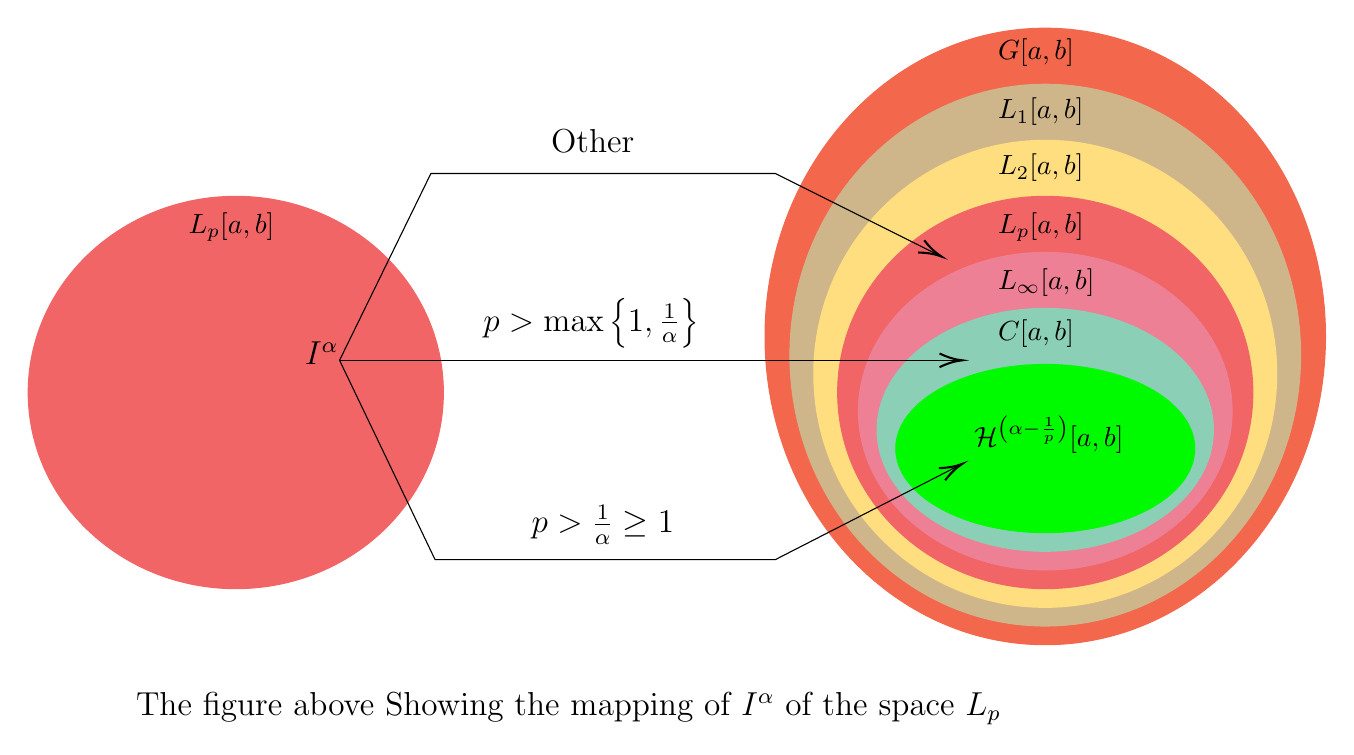
\begin{tikzpicture}[x=0.75pt,y=0.75pt,yscale=-1,xscale=1]
%uncomment if require: \path (0,757); %set diagram left start at 0, and has height of 757

%Shape: Ellipse [id:dp6907968999100429] 
\draw  [color={rgb, 255:red, 243; green, 103; blue, 77 }  ,draw opacity=1 ][fill={rgb, 255:red, 243; green, 103; blue, 77 }  ,fill opacity=1 ] (373.67,179.83) .. controls (373.67,97.82) and (434.11,31.33) .. (508.67,31.33) .. controls (583.23,31.33) and (643.67,97.82) .. (643.67,179.83) .. controls (643.67,261.85) and (583.23,328.33) .. (508.67,328.33) .. controls (434.11,328.33) and (373.67,261.85) .. (373.67,179.83) -- cycle ;
%Shape: Ellipse [id:dp455515408646161] 
\draw  [color={rgb, 255:red, 206; green, 182; blue, 138 }  ,draw opacity=1 ][fill={rgb, 255:red, 206; green, 182; blue, 138 }  ,fill opacity=1 ] (385.67,188.83) .. controls (385.67,116.76) and (440.74,58.33) .. (508.67,58.33) .. controls (576.6,58.33) and (631.67,116.76) .. (631.67,188.83) .. controls (631.67,260.91) and (576.6,319.33) .. (508.67,319.33) .. controls (440.74,319.33) and (385.67,260.91) .. (385.67,188.83) -- cycle ;
%Shape: Ellipse [id:dp45153781390969505] 
\draw  [color={rgb, 255:red, 255; green, 222; blue, 128 }  ,draw opacity=1 ][fill={rgb, 255:red, 255; green, 222; blue, 128 }  ,fill opacity=1 ] (397.17,197.83) .. controls (397.17,135.7) and (447.09,85.33) .. (508.67,85.33) .. controls (570.25,85.33) and (620.17,135.7) .. (620.17,197.83) .. controls (620.17,259.97) and (570.25,310.33) .. (508.67,310.33) .. controls (447.09,310.33) and (397.17,259.97) .. (397.17,197.83) -- cycle ;
%Shape: Ellipse [id:dp8046475401901105] 
\draw  [color={rgb, 255:red, 241; green, 101; blue, 103 }  ,draw opacity=1 ][fill={rgb, 255:red, 241; green, 101; blue, 103 }  ,fill opacity=1 ] (408.67,206.83) .. controls (408.67,154.64) and (453.44,112.33) .. (508.67,112.33) .. controls (563.9,112.33) and (608.67,154.64) .. (608.67,206.83) .. controls (608.67,259.02) and (563.9,301.33) .. (508.67,301.33) .. controls (453.44,301.33) and (408.67,259.02) .. (408.67,206.83) -- cycle ;
%Shape: Ellipse [id:dp6747974245031674] 
\draw  [color={rgb, 255:red, 238; green, 128; blue, 149 }  ,draw opacity=1 ][fill={rgb, 255:red, 238; green, 128; blue, 149 }  ,fill opacity=1 ] (418.67,215.83) .. controls (418.67,173.58) and (458.96,139.33) .. (508.67,139.33) .. controls (558.37,139.33) and (598.67,173.58) .. (598.67,215.83) .. controls (598.67,258.08) and (558.37,292.33) .. (508.67,292.33) .. controls (458.96,292.33) and (418.67,258.08) .. (418.67,215.83) -- cycle ;
%Shape: Ellipse [id:dp688684203224146] 
\draw  [color={rgb, 255:red, 139; green, 207; blue, 182 }  ,draw opacity=1 ][fill={rgb, 255:red, 139; green, 207; blue, 182 }  ,fill opacity=1 ] (427.67,224.83) .. controls (427.67,192.52) and (463.93,166.33) .. (508.67,166.33) .. controls (553.4,166.33) and (589.67,192.52) .. (589.67,224.83) .. controls (589.67,257.14) and (553.4,283.33) .. (508.67,283.33) .. controls (463.93,283.33) and (427.67,257.14) .. (427.67,224.83) -- cycle ;
%Shape: Ellipse [id:dp729097086157769] 
\draw  [color={rgb, 255:red, 0; green, 250; blue, 0 }  ,draw opacity=1 ][fill={rgb, 255:red, 0; green, 250; blue, 0 }  ,fill opacity=1 ] (436.67,233.83) .. controls (436.67,211.47) and (468.9,193.33) .. (508.67,193.33) .. controls (548.43,193.33) and (580.67,211.47) .. (580.67,233.83) .. controls (580.67,256.2) and (548.43,274.33) .. (508.67,274.33) .. controls (468.9,274.33) and (436.67,256.2) .. (436.67,233.83) -- cycle ;

%Shape: Ellipse [id:dp014732081794362362] 
\draw  [color={rgb, 255:red, 241; green, 101; blue, 103 }  ,draw opacity=1 ][fill={rgb, 255:red, 241; green, 101; blue, 103 }  ,fill opacity=1 ] (18.67,206.83) .. controls (18.67,154.64) and (63.44,112.33) .. (118.67,112.33) .. controls (173.9,112.33) and (218.67,154.64) .. (218.67,206.83) .. controls (218.67,259.02) and (173.9,301.33) .. (118.67,301.33) .. controls (63.44,301.33) and (18.67,259.02) .. (18.67,206.83) -- cycle ;
%Straight Lines [id:da35032145832073125] 
\draw    (168.67,191.33) -- (212.67,101.33) -- (378.67,101.33) -- (456.88,140.44) ;
\draw [shift={(458.67,141.33)}, rotate = 206.57] [color={rgb, 255:red, 0; green, 0; blue, 0 }  ][line width=0.75]    (10.93,-3.29) .. controls (6.95,-1.4) and (3.31,-0.3) .. (0,0) .. controls (3.31,0.3) and (6.95,1.4) .. (10.93,3.29)   ;
%Straight Lines [id:da6570360584697525] 
\draw    (168.67,191.33) -- (466.67,191.33) ;
\draw [shift={(468.67,191.33)}, rotate = 180] [color={rgb, 255:red, 0; green, 0; blue, 0 }  ][line width=0.75]    (10.93,-3.29) .. controls (6.95,-1.4) and (3.31,-0.3) .. (0,0) .. controls (3.31,0.3) and (6.95,1.4) .. (10.93,3.29)   ;
%Straight Lines [id:da6760674585190951] 
\draw    (168.67,191.33) -- (214.67,287.33) -- (378.67,287.33) -- (466.89,242.13) ;
\draw [shift={(468.67,241.22)}, rotate = 152.87] [color={rgb, 255:red, 0; green, 0; blue, 0 }  ][line width=0.75]    (10.93,-3.29) .. controls (6.95,-1.4) and (3.31,-0.3) .. (0,0) .. controls (3.31,0.3) and (6.95,1.4) .. (10.93,3.29)   ;

% Text Node
\draw (94.67,118.73) node [anchor=north west][inner sep=0.75pt]    {$L_{p}[ a,b]$};
% Text Node
\draw (484.67,35.23) node [anchor=north west][inner sep=0.75pt]    {$G[ a,b]$};
% Text Node
\draw (484.67,63.73) node [anchor=north west][inner sep=0.75pt]    {$L_{1}[ a,b]$};
% Text Node
\draw (484.67,90.73) node [anchor=north west][inner sep=0.75pt]    {$L_{2}[ a,b]$};
% Text Node
\draw (484.67,145.73) node [anchor=north west][inner sep=0.75pt]    {$L_{\infty }[ a,b]$};
% Text Node
\draw (484.67,118.73) node [anchor=north west][inner sep=0.75pt]    {$L_{p}[ a,b]$};
% Text Node
\draw (484.67,170.73) node [anchor=north west][inner sep=0.75pt]    {$C[ a,b]$};
% Text Node
\draw (473.17,216.73) node [anchor=north west][inner sep=0.75pt]    {$\mathcal{H}^{\left( \alpha -\frac{1}{p}\right)}[ a,b]$};
% Text Node
\draw (236.67,160) node [anchor=north west][font=\large,inner sep=0.75pt]    {$p >\max\left\{1,\frac{1}{\alpha }\right\}$};
% Text Node
\draw (260,260) node [anchor=north west][font=\large,inner sep=0.75pt]    {$p >\frac{1}{\alpha} \geq 1$};
% Text Node
\draw (150.67,180.96) node [anchor=north west][font=\large,inner sep=0.75pt]    {$I^{\alpha }$};
% Text Node
\draw (269.33,79) node [anchor=north west][font=\large,inner sep=0.75pt]   [align=left] {Other};
\draw (69.33,350) node [anchor=north west][font=\large,inner sep=0.75pt]   [align=left] {The figure above Showing the mapping of $I^{\alpha}$ of the space $L_p$};
\end{tikzpicture}
% }
\end{center}
% Where
% \begin{itemize}
%     \item $G(a,b)$ the space of all bounded functions on $[a,b]$
%     \item $L_1[a,b]$ the space of absolutely integrable functions on $[a,b]$
%     \[
%         \int_{a}^{b} f(t) dt < \infty \implies f(t) \in L_1[a,b]
%     \]
%     \item $L_2[a,b]$ also known as Hilbert space, the space of square-integrable functions on $[a,b]$
%     \[
%         \left( \int_{a}^{b} \left( f(t) \right)^2 dt \right)^{\frac{1}{2}} < \infty \implies f(t) \in L_2[a,b]
%     \]
%     \item $L_p[a,b]$ the space of p-integrable functions on $[a,b]$
%     \[
%         \left( \int_{a}^{b} \left( f(t) \right)^p dt \right)^{\frac{1}{p}} < \infty \implies f(t) \in L_p[a,b]
%     \]
%     \item $L_\infty[a,b]$ the space of essentially bounded measurable functions on $[a,b]$
%     \item $C[a,b]$ the space of continuous functions on $[a,b]$
%     \item $\mathcal{H}^{\lambda}[a,b]$ the space of Holderian functions of order $\lambda$ on $[a,b]$
% \end{itemize}

% \[
%     G(a,b) \supset  L_1[a,b] \supset L_2[a,b] \supset L_p[a,b]  \supset L_\infty[a,b] \supset C[a,b] \supset \mathcal{H}^{\lambda}[a,b]
% \]